\section{Ergebnisse}
\subsection{Standardwerte}
\begin{frame}{Standardwerte}
	\begin{itemize}[<+->]
		\item Feature Extraction
		\begin{itemize}[<1->]
			\item 32 ms Fenster
			\item Halber Vorschub
			\item 90 \% Energielevel
			\item 12 Merkmale (LPC) bzw. 20 Merkmale (MFCC)
		\end{itemize}
		\item Neural Gas
		\begin{itemize}[<1->]
			\item 100 Prototypen
			\item 15 Iterationen
		\end{itemize}
		\item SVM
		\begin{itemize}[<1->]
			\item RBF bzw. linearer Kernel
			\item $\gamma$ = 1
			\item c = 1
		\end{itemize}
	\end{itemize} 
\end{frame}

\subsection{Vergleich}
\begin{frame}{Vergleich}
	\begin{center}		
		\begin{tabular}{l|c|c}			
			& LPC & MFCC \\
			\hline
			Neural Gas & 40 \% & 71 \% \\
			SVM (linear) & 46 \% & 72 \% \\
			SVM (RBF) & 54 \% & 80 \% \\
		\end{tabular}
	\end{center}
	\begin{center}
		Erkennungsrate auf Einzelframes
	\end{center}	
\end{frame}

\begin{frame}{LPC - Neural Gas}
	\begin{center}
		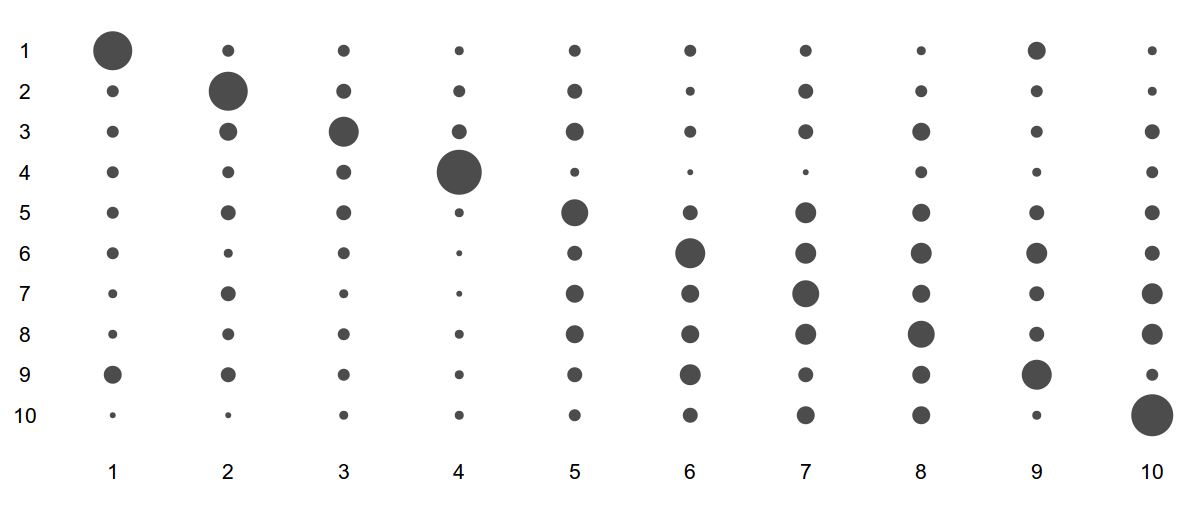
\includegraphics[width=1.0\textwidth]{img/lpcNgMatrix}
	\end{center}
	\begin{center}
		Durchschnittliche Erkennungsrate: 40,09 \%
	\end{center}
\end{frame}

\begin{frame}{MFCC - Neural Gas}
	\begin{center}
		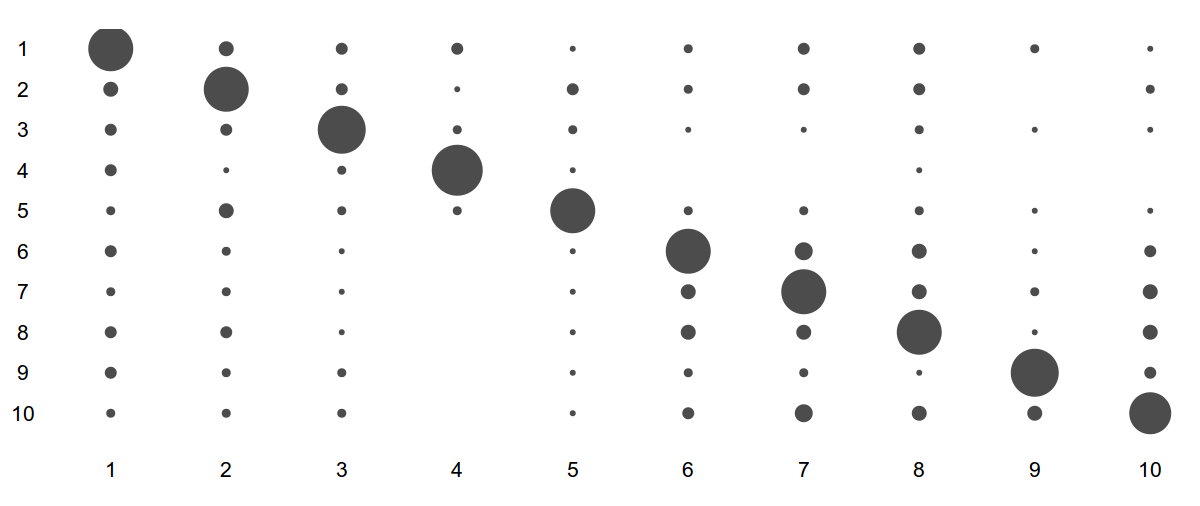
\includegraphics[width=1.0\textwidth]{img/mfccNgMatrix}
	\end{center}
	\begin{center}
		Durchschnittliche Erkennungsrate: 71,25 \%
	\end{center}
\end{frame}

\begin{frame}{MFCC - SVM (RBF)}
	\begin{center}
		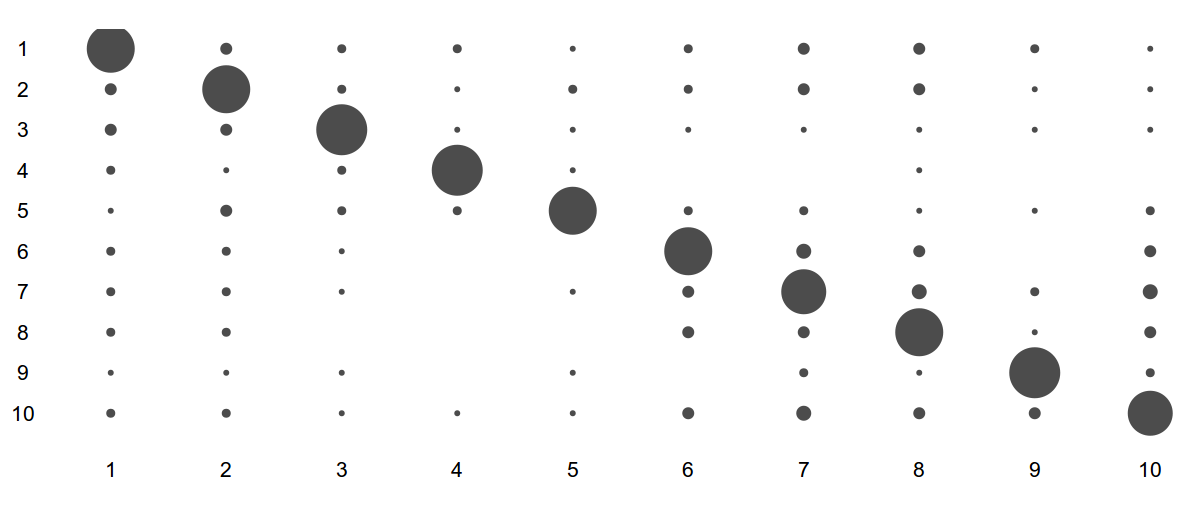
\includegraphics[width=1.0\textwidth]{img/mfccSvmRbfMatrix}
	\end{center}
	\begin{center}
		Durchschnittliche Erkennungsrate: 80,44 \%
	\end{center}
\end{frame}

\subsection{Optimierung}
\begin{frame}{Optimierung (Evolutionärer Algorithmus)}
	\begin{itemize}[<+->]
		\item Optimierung der Parameter von MFCC und Neural Gas
		\item variable Mutationsrate
		\item Fitnessfunktion $\begin{aligned}[t]f(t,acc) = \frac{acc}{1 - e^{\left(\frac{-t}{1000}\right)}}\end{aligned}$
		\begin{itemize}[<1->]
			\item t = Zeit in Sekunden
			\item acc = Erkennungsrate in Prozent
		\end{itemize}
		\item Tournament-Selektion
	\end{itemize}		
\end{frame}

\begin{frame}{Ergebnisse durch Optimierung}
	\begin{center}
		\hspace*{-8mm}
		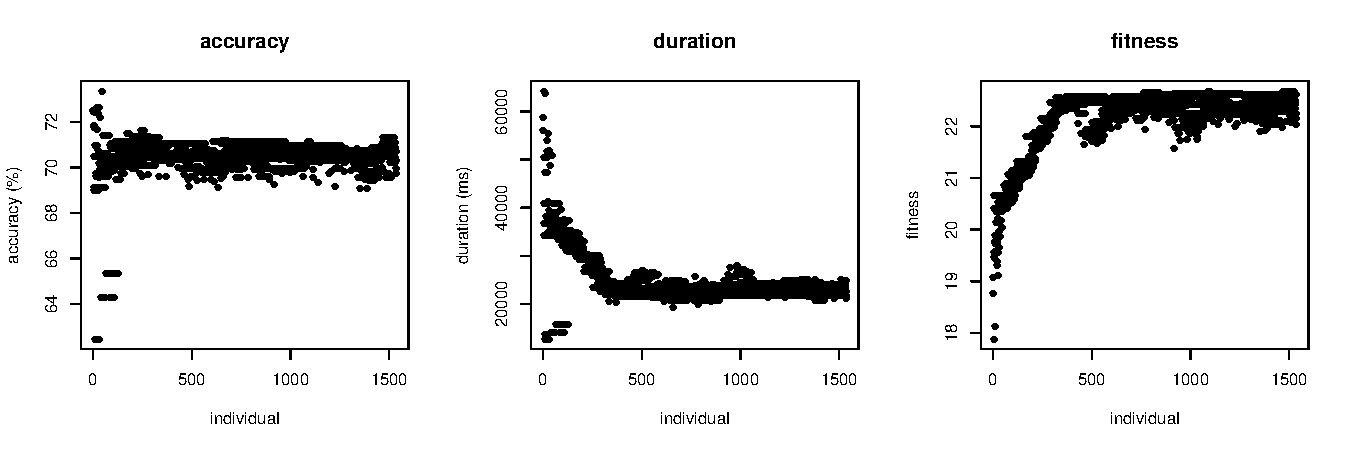
\includegraphics[width=1.15\textwidth]{img/eaFitness}
	\end{center}
\end{frame}

\begin{frame}{Ergebnisse durch Optimierung}
	\begin{columns}
		\column{0.55\linewidth}
		\begin{itemize}
			\item MFCC
			\begin{itemize}[<1->]
				\item 32 ms Fenster (fix)
				\item 100 \% \ding{222} 20 \% Vorschub
				\item 96 \% \ding{222} 85 \% Energielevel
				\item 25 - 33 Merkmale
			\end{itemize}
			\item Neural Gas
			\begin{itemize}[<1->]
				\item 53 \ding{222} 176 Prototypen
				\item 5 \ding{222} 9 Iterationen
			\end{itemize}
		\end{itemize}
		\column{0.45\linewidth}
		\begin{center}
			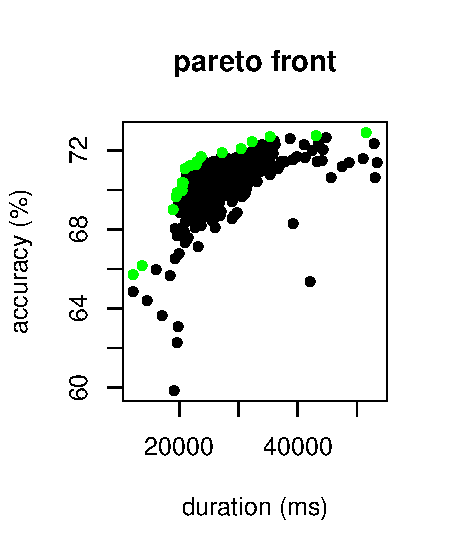
\includegraphics[width=1.0\textwidth]{img/eaPareto}
		\end{center} 
	\end{columns}
\end{frame}
